%%%%%%%%%%%%%%%%%%%%%%%%%%%%%%%%%%%%%%%%%%%%%%%%%%%%%%%%%%%%%%%%%%%%%%%%%%%%%%%
\subsection{Introduction}
%%%%%%%%%%%%%%%%%%%%%%%%%%%%%%%%%%%%%%%%%%%%%%%%%%%%%%%%%%%%%%%%%%%%%%%%%%%%%%%

%%%%%%%%%%%%%%%%%%%%%%%%%%%%%%%%%%%%%%%%%%%%%%%%%%%%%%%%%%%%%%%%%%%%%%%%%%%%%%%
%%%%%%%%%%%%%%%%%%%%%%%%%%%%%%%%%%%%%%%%%%%%%%%%%%%%%%%%%%%%%%%%%%%%%%%%%%%%%%%
%%%%%%%%%%%%%%%%%%%%%%%%%%%%%%%%%%%%%%%%%%%%%%%%%%%%%%%%%%%%%%%%%%%%%%%%%%%%%%%
\begin{frame}{Why \LaTeX{}?}
    \begin{itemize}
        \item It makes beautiful documents
              \begin{itemize}
                  \item Especially mathematics
              \end{itemize}
              %
        \item It was created by scientists, for scientists
              \begin{itemize}
                  \item A large and active community
              \end{itemize}
              %
        \item It is powerful --- you can extend it
              \begin{itemize}
                  \item Packages for papers, presentations, spreadsheets, \ldots
              \end{itemize}
    \end{itemize}
\end{frame}

%%%%%%%%%%%%%%%%%%%%%%%%%%%%%%%%%%%%%%%%%%%%%%%%%%%%%%%%%%%%%%%%%%%%%%%%%%%%%%%
%%%%%%%%%%%%%%%%%%%%%%%%%%%%%%%%%%%%%%%%%%%%%%%%%%%%%%%%%%%%%%%%%%%%%%%%%%%%%%%
%%%%%%%%%%%%%%%%%%%%%%%%%%%%%%%%%%%%%%%%%%%%%%%%%%%%%%%%%%%%%%%%%%%%%%%%%%%%%%%
\begin{frame}[fragile]{How does it work?}
    \begin{itemize}
        \item You write your document in \texttt{plain text} with \cmd{commands} that
              describe its structure and meaning.
        \item The \texttt{latex} program processes your text and commands to produce a
              beautifully formatted document.
    \end{itemize}
    \vskip 2ex
    \begin{center}
        \begin{lstlisting}
        The rain in Spain falls \emph{mainly} on the plain.
    \end{lstlisting}
        \vskip 2ex
        \tikz\node[single arrow,fill=gray,font=\ttfamily\bfseries,%
            rotate=270,xshift=-1em]{latex};
        \vskip 2ex
        \fbox{The rain in Spain falls \emph{mainly} on the plain.}
    \end{center}
\end{frame}

% %%%%%%%%%%%%%%%%%%%%%%%%%%%%%%%%%%%%%%%%%%%%%%%%%%%%%%%%%%%%%%%%%%%%%%%%%%%%%%%
% %%%%%%%%%%%%%%%%%%%%%%%%%%%%%%%%%%%%%%%%%%%%%%%%%%%%%%%%%%%%%%%%%%%%%%%%%%%%%%%
% %%%%%%%%%%%%%%%%%%%%%%%%%%%%%%%%%%%%%%%%%%%%%%%%%%%%%%%%%%%%%%%%%%%%%%%%%%%%%%%
\begin{frame}[fragile]{More examples of commands and their output\ldots}

    \begin{figure}[h]
        \centering
        \begin{minipage}{0.5\textwidth}
            % 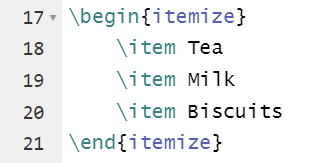
\includegraphics[width=0.3\textheight]{figs/itemize_basic.png}
            \begin{lstlisting}[showlines=true]
\begin{itemize}
    \item Tea
    \item Milk
    \item Biscuits
\end{itemize}
            \end{lstlisting}
        \end{minipage}
        \begin{minipage}{0.4\textwidth}
            \begin{itemize}
                \item Tea
                \item Milk
                \item Biscuits
            \end{itemize}
        \end{minipage}
    \end{figure}

    % \vskip 2ex

    \begin{figure}[h]
        \centering
        \begin{minipage}{0.5\textwidth}
            % 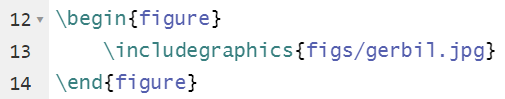
\includegraphics[width=0.5\textwidth]{figs/includegraphics_basic.png}
            \begin{lstlisting}
\begin{figure}
    \centering
    
\includegraphics{figs/gerbil.jpg}
\end{figure}
            \end{lstlisting}
        \end{minipage}
        \begin{minipage}{0.4\textwidth}
            
\includegraphics[width=0.25\textwidth]{figs/gerbil.jpg}
        \end{minipage}
    \end{figure}

    % \vskip 2ex

    \begin{figure}
        % \centering
        \begin{minipage}{0.5\textwidth}
            % 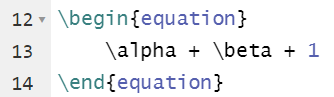
\includegraphics[width=0.4\textwidth]{figs/equation_basic.png}
            \begin{lstlisting}
\begin{equation}
    \alpha + \beta + 1
\end{equation}
            \end{lstlisting}
        \end{minipage}
        \begin{minipage}{0.4\textwidth}
            \begin{equation}
                \alpha + \beta + 1
            \end{equation}
        \end{minipage}
    \end{figure}

\end{frame}

%%%%%%%%%%%%%%%%%%%%%%%%%%%%%%%%%%%%%%%%%%%%%%%%%%%%%%%%%%%%%%%%%%%%%%%%%%%%%%%
\subsection{Quick Tips}
%%%%%%%%%%%%%%%%%%%%%%%%%%%%%%%%%%%%%%%%%%%%%%%%%%%%%%%%%%%%%%%%%%%%%%%%%%%%%%%

%%%%%%%%%%%%%%%%%%%%%%%%%%%%%%%%%%%%%%%%%%%%%%%%%%%%%%%%%%%%%%%%%%%%%%%%%%%%%%%
%%%%%%%%%%%%%%%%%%%%%%%%%%%%%%%%%%%%%%%%%%%%%%%%%%%%%%%%%%%%%%%%%%%%%%%%%%%%%%%
%%%%%%%%%%%%%%%%%%%%%%%%%%%%%%%%%%%%%%%%%%%%%%%%%%%%%%%%%%%%%%%%%%%%%%%%%%%%%%%
\begin{frame}[fragile]{Attitude adjustment}

    \begin{itemize}
        \item Use commands to describe `what it is', not `how it looks'.
        \item Focus on your content.
        \item Let \LaTeX{} do its job.
    \end{itemize}
\end{frame}


%%%%%%%%%%%%%%%%%%%%%%%%%%%%%%%%%%%%%%%%%%%%%%%%%%%%%%%%%%%%%%%%%%%%%%%%%%%%%%%
%%%%%%%%%%%%%%%%%%%%%%%%%%%%%%%%%%%%%%%%%%%%%%%%%%%%%%%%%%%%%%%%%%%%%%%%%%%%%%%
%%%%%%%%%%%%%%%%%%%%%%%%%%%%%%%%%%%%%%%%%%%%%%%%%%%%%%%%%%%%%%%%%%%%%%%%%%%%%%%
\begin{frame}[fragile]{Caveats}
    \small
    \begin{itemize}
        \item Quotation marks are a bit tricky:\\
              use a backtick \keystroke{\`{}} on the left and an apostrophe \keystroke{\'{}} on the right.
              \begin{tabular}{rcl}
                  Single Quotes: & \verb|`text'|   & `text'   \\
                  Double Quotes: & \verb|``text''| & ``text''
              \end{tabular}

        \item Some common characters have special meanings in \LaTeX:
              \\[1ex]
              \begin{tabular}{rcl}
                  \keystrokebftt{\%} & percent sign              & \verb|\%| \\
                  \keystrokebftt{\#} & hash (pound / sharp) sign & \verb|\&| \\
                  \keystrokebftt{\&} & ampersand                 & \verb|\&| \\
                  \keystrokebftt{\$} & dollar sign               & \verb|\$|
              \end{tabular}
        \item If you just type these, you'll get an error. If you want one to appear in the output, you have to \emph{escape} it by preceding it with a backslash.
    \end{itemize}
\end{frame}

%%%%%%%%%%%%%%%%%%%%%%%%%%%%%%%%%%%%%%%%%%%%%%%%%%%%%%%%%%%%%%%%%%%%%%%%%%%%%%%
%%%%%%%%%%%%%%%%%%%%%%%%%%%%%%%%%%%%%%%%%%%%%%%%%%%%%%%%%%%%%%%%%%%%%%%%%%%%%%%
%%%%%%%%%%%%%%%%%%%%%%%%%%%%%%%%%%%%%%%%%%%%%%%%%%%%%%%%%%%%%%%%%%%%%%%%%%%%%%%
\begin{frame}[fragile]{Handling Errors}
    \begin{itemize}
        \item \LaTeX{} can get confused when it is trying to compile your document. If
              it does, it stops with an error, which you must fix before it will produce
              any output.
        \item For example, if you misspell \cmdbs{emph} as \cmdbs{meph}, \LaTeX{} will
              stop with an ``undefined control sequence'' error, because ``meph'' is not
              one of the commands it knows.
    \end{itemize}
    \begin{block}{Advice on Errors}
        \begin{enumerate}
            \item Don't panic! Errors happen.
            \item Fix them as soon as they arise --- if what you just typed caused an error,
                  you can start your debugging there.
            \item If there are multiple errors, start with the first one --- the cause may
                  even be above it.
        \end{enumerate}
    \end{block}
\end{frame}

%%%%%%%%%%%%%%%%%%%%%%%%%%%%%%%%%%%%%%%%%%%%%%%%%%%%%%%%%%%%%%%%%%%%%%%%%%%%%%%
\subsection{Documentation and Resources}
%%%%%%%%%%%%%%%%%%%%%%%%%%%%%%%%%%%%%%%%%%%%%%%%%%%%%%%%%%%%%%%%%%%%%%%%%%%%%%%

\begin{frame}
    \frametitle{Overleaf: Online editor and great Documentation}

      

\end{frame}